\documentclass{article}
\usepackage{amsmath}
\usepackage[margin=1.5cm]{geometry}
\usepackage{pgfplots}
\pgfplotsset{width=10cm,compat=1.9}
\begin{document}

\begin{center}
	\title{Algebra Basics}
\end{center}

\section{Percent Increase}
\textbf{Calculate the final price of the given item}

\bigskip

\(\begin{aligned}
	&Original: \$80; Tax: 3\%  \qquad\qquad Original: \$129.95; Tax: 6\% \\\\
	&Original: \$99.50; Markup: 15\% \qquad\qquad	 Original: \$0.95; Markup: 80\% \\\\
\end{aligned}\)

\section{Percent Decrease}
\textbf{Calculate the final price of the item}

\bigskip

\(\begin{aligned}
	&Original: \$17.50; Discount: 20\%  \qquad Original: \$299.99; Discount: 15\% \\\\
	&Original: \$60; Discount: 12\% \qquad	 Original: \$1.49; Discount: 30\% \\\\
\end{aligned}\)

\section{percent Change}
\textbf{Calculate the percent change and indicate whether it was an increase or decrease}

\bigskip

\(\begin{aligned}
	&Original: \$28; Final: \$37.24  \qquad\qquad Original: 316,000; Final: 309,680 \\\\
	&Original: \$100; Final: \$108 \qquad\qquad	 Original: \$21; Final: \$22.05 \\\\
	&Original: 209,000; Final: 217,360 \qquad\qquad	 Original: \$200; Final: \$216 \\\\
\end{aligned}\)

\section{Simple Interest}
\textbf{Find the total cost of the item including interest}

\bigskip

\(\begin{aligned}
	&Price: \$20,000; \:\ Rate: 4.99\%;\:\ Time: 5\ years  \\\\
	&Price: \$540,000;\:\ Rate: 6.25\%;\:\ Time: 30\ years \\\\
\end{aligned}\)

\section{Functions}
\textbf{Evaluate the functions for the given inputs}
\bigskip

\(\begin{aligned}
	&f(x)=2x+3;\: f(7) \qquad g(x)=13x-4;\: g(8) \qquad f(x)=5(7-x)+2;\: f(-3)\\\\
	&f(x)=\frac{3}{5}x+\frac{1}{2};\: f(\frac{1}{2})\qquad g(x)=\frac{2x-5}{3};\: g(y+7) \qquad f(x)=\frac{3}{15x+2};\: f(0)\\\\
	&f(x)=12x-9; \:f(y) \qquad g(x)=6x-4; \:g(\frac{1}{2}y) \qquad f(x)=-3(x+7);\: f(y^2)\\\\
	&f(x)=x^2+3; \:f(5) \qquad g(x)=x^3+x^2-x;\: g(-1) \qquad f(x)=(x+7)^2;\: f(3)\\\\
\end{aligned}\)

\section{The Vertical Line Test}
\textbf{Declare whether or not the given plot is a function}

\bigskip

\begin{tikzpicture}
\begin{axis}[
    xmin=-4,xmax=4,
    ymin=-4,ymax=4,
    enlargelimits={abs=0},
    axis lines=middle,
    axis line style={latex-latex},
	ticks=none,
    xlabel style={at={(ticklabel* cs:1)},anchor=north west},
	ylabel style={at={(ticklabel* cs:1)},anchor=south west},
	width=150]
	\addplot[domain=0:2*pi, samples=100, thick, red] ({cos(deg(x))}, {sin(deg(x))});
\end{axis}
\end{tikzpicture}
\qquad\qquad
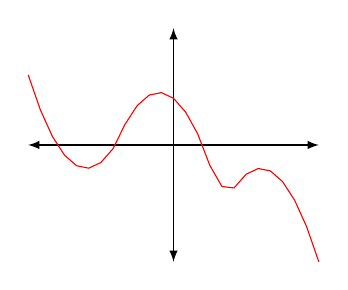
\begin{tikzpicture}[
  declare function={
    func(\x)= (\x<=-2) * (\x*\x + 6*\x + 8)   +
     and(\x>-2, \x<=1) * (2 - \x - \x*\x)     +
     and(\x>1,  \x<=2) * (6 - 8*\x + 2*\x*\x) +
                (\x>2) * (-10 + 6*\x - \x*\x);
  }
]
\begin{axis}[
  axis x line=middle, axis y line=middle,
    axis line style={latex-latex},
  ymin=-5, ymax=5, 
  xmin=-5, xmax=5,
	width=150,
	ticks=none,
	clip=false,
]

	\addplot[red,domain=-5:5]{func(x)};
\end{axis}
\end{tikzpicture}

\bigskip

\begin{tikzpicture}
\begin{axis}[
  axis x line=middle, axis y line=middle,
    axis line style={latex-latex},
  ymin=-5, ymax=5, 
  xmin=-5, xmax=5,
	width=150,
	ticks=none,
	clip=false,
]
\qquad\qquad
	\addplot[style={latex-latex}, red] coordinates {(1,-5) (1,5)};
	%\addplot{x=2};
\end{axis}
\end{tikzpicture} 
\qquad\qquad
\begin{tikzpicture}
\begin{axis}[
    samples=6, % Total points (10-0+1)
  axis x line=middle, axis y line=middle,
    axis line style={latex-latex},
  ymin=-5, ymax=5, 
  xmin=-5, xmax=5,
	width=150,
	ticks=none,
	clip=false,
]
    ]
    % Use 'only marks' for dots
    \addplot [only marks, mark=*, red] {sin(deg(x))};
\end{axis}
\end{tikzpicture}

\bigskip



\section{Plotting Points}
\textbf{Plot and label the following points}

\bigskip

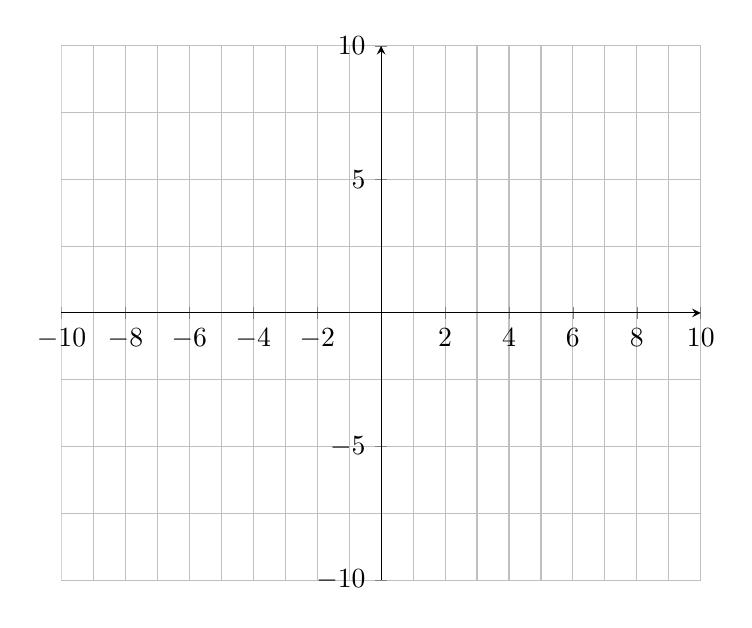
\begin{tikzpicture}
	\begin{axis}[width=0.8\linewidth,
		axis lines=middle, 
		grid=both, ymin=-10, ymax=10,
		%ytick=({-10,-9,...,10},
		minor tick num=1,
		minor tick style={draw=none},
		xmin=-10, xmax=10,
		%xtick={-10,-9,...,10},
		xticklabel={ },
		%xticklabel style={rotate=45,anchor=north east}
		]
		\addplot[draw=none] coordinates{(1,1)};
	\end{axis}
\end{tikzpicture}

\section{Domain and Range}
\section{Additive Equations}
\textbf{Solve for the given variable}

\bigskip

\(\begin{aligned}
	&x+4=10 \qquad\qquad 6-y=-4 \qquad\qquad 13+z=9 \qquad\qquad 9.7+x=12.3 \qquad\qquad -x-800=97\\\\
	&y+\frac{3}{5}=1 \qquad\qquad -\frac{7}{3}-z=\frac{11}{3} \qquad\qquad x+\frac{2}{5}=\frac{1}{4} \qquad\qquad  x+3\frac{1}{5}=15\frac{1}{2} \qquad\qquad \frac{8}{5}-x=1\frac{3}{5}\\\
\end{aligned}\)
\section{Additive Inequalities}
\textbf{Solve for the given variable}

\bigskip

\(\begin{aligned}
	&x-3>9 \qquad\qquad 4<x-1 \qquad\qquad -1\ge-11+x \qquad\qquad -20\ge10x \qquad\qquad x-\frac{1}{2} <0\\\\
\end{aligned}\)

\section{Multiplicative Equations}
\textbf{Solve for the given variable}

\bigskip

\(\begin{aligned}
	&-50=10b \qquad\qquad 8n=-48 \qquad\qquad 60=-12w \qquad\qquad  12x=9 \qquad\qquad -15=-9s\\\\
	&-7=4x \qquad\qquad 10=4x \qquad\qquad \frac{x}{-7}=9 \qquad\qquad -6=\frac{n}{9} \qquad\qquad \frac{-s}{8}=-1 \qquad\qquad -\frac{4}{3}y=-6\\\\
\end{aligned}\)

\section{Multiplicative Inequalities}
\section{Two-Step Equations}
\section{Two-Step Inequalities}
\section{Plotting Points}
\section{Slope-Intercept Form}
\section{Standard Form}


\end{document}

